\chapter{Progress and Expected Contributions}

\section{Work Completed}

Since the submission of the initial proposal, substantial progress has been achieved across the theoretical, implementation, and evaluation components of the project.

\begin{enumerate}
    \item \textbf{Formal correctness proofs for PF-A*.}
          The admissibility and consistency of $h_{\mathrm{PF}}(v,f)$ have been formally established in Chapter~\ref{ch:correctness}, thereby addressing the principal theoretical limitation identified during the proposal stage.
          These results demonstrate that PF-A* constitutes a provably correct optimal heuristic extension of RF-A*, rather than a purely empirical refinement.

    \item \textbf{Implementation of the algorithmic framework.}
          Six algorithms have been implemented: State-Expanded Dijkstra, Greedy, DP, Standard A*, RF-A*, and PF-A*.
          Their correctness has been validated through a unit testing framework using both the running example and an additional set of 50 hand-crafted graphs.

    \item \textbf{Construction of the real-world Thai dataset.}
          The real-world dataset required for evaluation has been assembled by integrating fuel station geographic coordinates, road network topology, and provincial fuel price information from the relevant data sources.
          In addition, the three target evaluation corridors, Bangkok--Chiang Mai, Bangkok--Phuket, and Bangkok--Khon Kaen, have been prepared for experimental use.

    \item \textbf{Development of the synthetic benchmark generator.}
          A configurable synthetic benchmark generator has been implemented and validated in accordance with the parameter settings defined in Table~\ref{tab:synth_params}.

    \item \textbf{Execution of preliminary synthetic experiments and visualisation pipeline.}
          The synthetic experiment suite described in Chapter~\ref{ch:experiments} has been executed in a reduced but repeatable smoke-profile configuration and integrated with an automated analysis pipeline.
          This workflow now covers benchmark generation, algorithm execution, result recording, summary-table generation, and figure production.
          The resulting charts and tables have been incorporated into Section~\ref{sec:prelim_results}, replacing the earlier placeholder discussion.
\end{enumerate}

\section{Current Synthetic Results and Analysis}
\label{sec:prelim_results}

This section updates the progress report with the actual synthetic results currently available in the repository.
The experiments were executed from the Windows benchmarking harness using the smoke profile, with 10 timed runs per configuration, 0 warm-up runs, base graph size 100 nodes, scalability sizes 100 and 1000 nodes, degree 5, tank capacity 40\,L unless otherwise varied, initial fuel 28\,L unless otherwise varied, and efficiency 10\,km/L.
The resulting dataset contains 1,460 timed runs across Experiments~1, 2, 3, 4, 5, and~7.

Although this is still a reduced profile relative to the final dissertation target of 10,000 timed runs and 200 warm-up iterations per configuration, the present results are now sufficient to support a substantive empirical analysis of the implemented synthetic pipeline.
They also provide clear direction for the remaining real-world evaluation in Experiment~6.

\begin{table}[H]
    \centering
    \caption{Current synthetic execution profile used for the updated progress report.}
    \label{tab:current_synth_profile}
    \begin{tabular}{ll}
        \toprule
        Setting & Value \\
        \midrule
        Timed runs per configuration & 10 \\
        Warm-up runs per configuration & 0 \\
        Base graph size & 100 nodes \\
        Scalability graph sizes & 100, 1000 nodes \\
        Approximate degree & 5 \\
        Default tank capacity & 40\,L \\
        Default initial fuel & 28\,L \\
        Fuel efficiency & 10\,km/L \\
        Total result rows & 1,460 \\
        Covered experiments & 1, 2, 3, 4, 5, and 7 \\
        \bottomrule
    \end{tabular}
\end{table}

\subsection*{Experiment 1: Scalability}

The scalability results already show a strong practical separation between the exact methods and the heuristic methods.
At 1000 nodes, State-Expanded Dijkstra required 1771.17\,ms on average and Dynamic Programming required 1640.96\,ms, whereas PF-A* completed in 552.37\,ms while matching the same mean cost of 2876.88.
This makes PF-A* approximately 3.2$\times$ faster than Dijkstra and about 3.0$\times$ faster than Dynamic Programming on the largest currently executed synthetic graph.
By contrast, Standard A* and RF-A* were both much slower, exceeding 5.3\,s on average at 1000 nodes.
Greedy remained infeasible in both tested graph sizes, so it currently serves only as a weak baseline rather than a competitive method.

\begin{table}[H]
    \centering
    \caption{Experiment~1 summary at 1000 nodes.}
    \label{tab:exp1_summary_1000}
    \begin{tabular}{lccc}
        \toprule
        Algorithm & Feasible (\%) & Mean Cost & Mean Runtime (ms) \\
        \midrule
        State-Expanded Dijkstra & 100 & 2876.88 & 1771.17 \\
        Dynamic Programming & 100 & 2876.88 & 1640.96 \\
        Greedy & 0 & --- & 855.50 \\
        Standard A* & 100 & 2933.71 & 5359.22 \\
        RF-A* & 100 & 2933.71 & 5381.99 \\
        PF-A* & 100 & 2876.88 & 552.37 \\
        \bottomrule
    \end{tabular}
\end{table}

\begin{figure}[H]
      \centering
      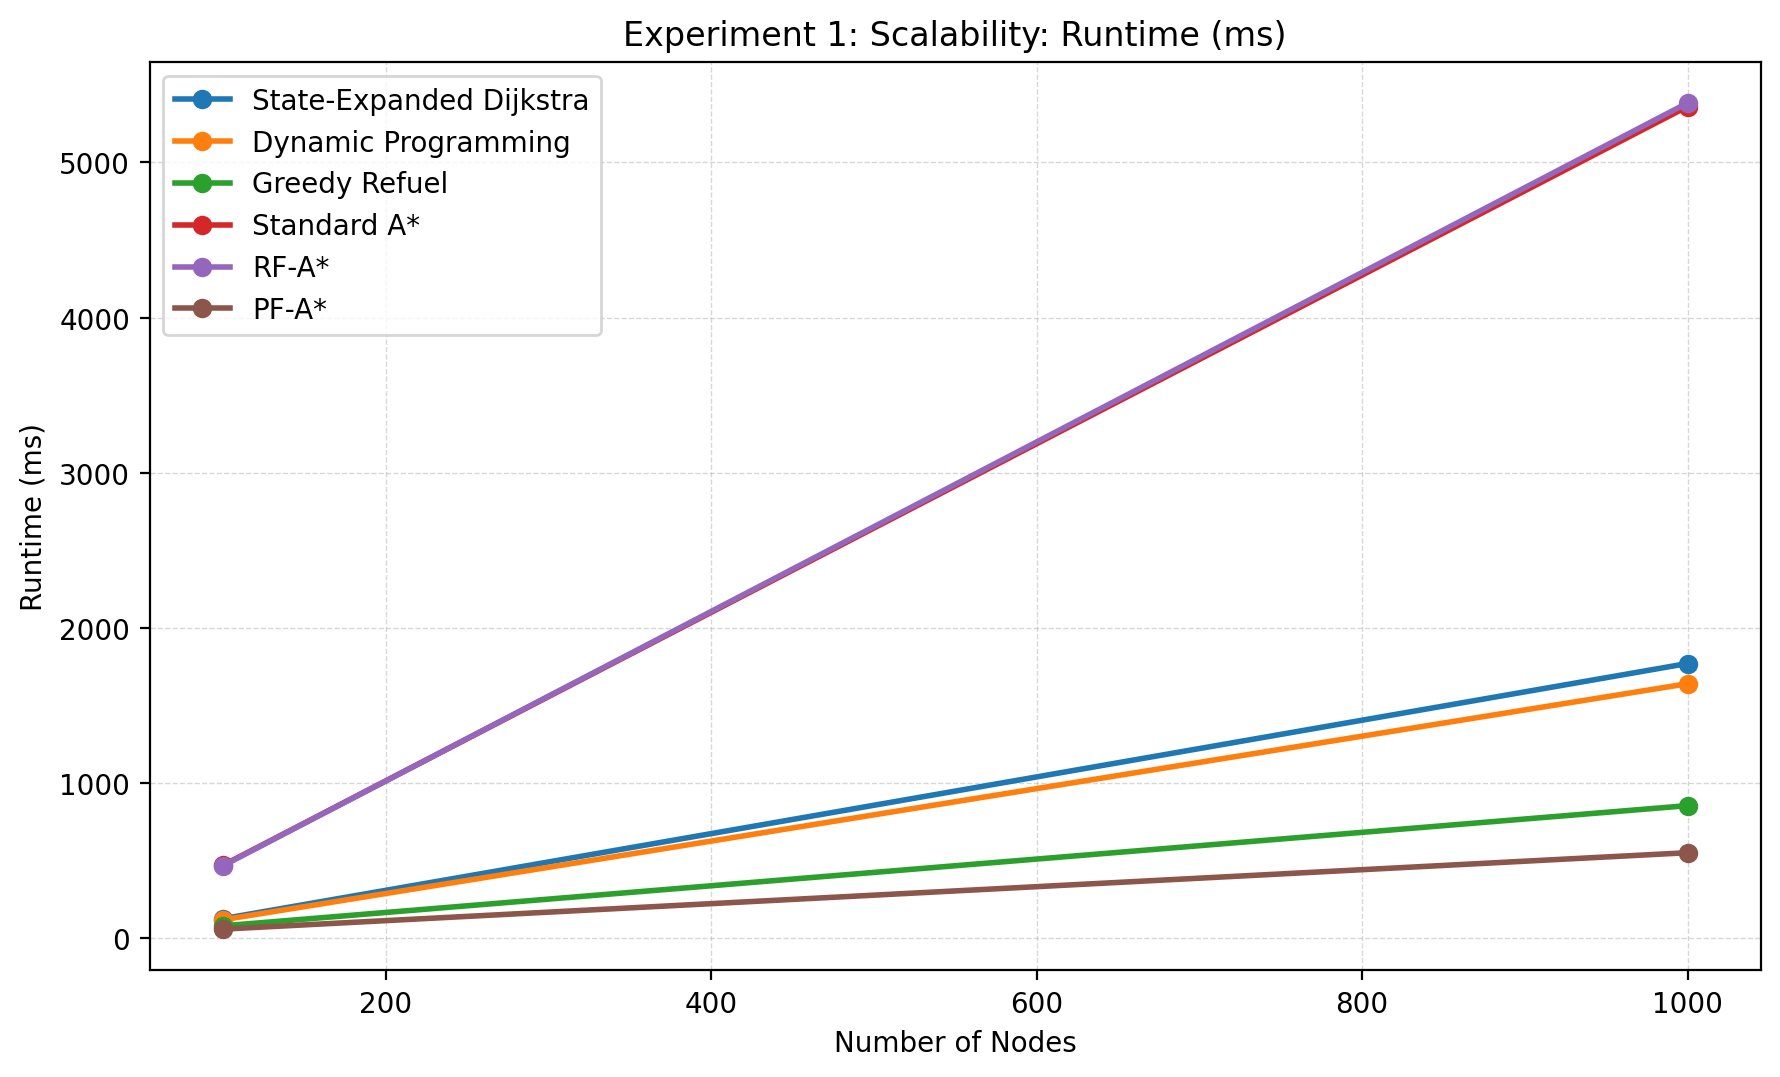
\includegraphics[width=0.90\textwidth]{../results/report_assets/exp1_scalability/exp1_scalability_runtime.png}
      \caption{Experiment~1 runtime as graph size increases. PF-A* scales substantially better than the exact Dijkstra and Dynamic Programming baselines in the current synthetic profile, while remaining much faster than Standard A* and RF-A*.}
      \label{fig:curr_exp1_runtime}
\end{figure}

\subsection*{Experiment 2: Fuel Price Variance}

Experiment~2 shows that increasing fuel-price variance makes price-aware routing materially more valuable.
The optimal mean cost, as represented by State-Expanded Dijkstra, Dynamic Programming, and PF-A*, fell from 3528.00 at $\sigma=0\%$ to 2576.21 at $\sigma=20\%$.
This confirms the expected intuition that larger price dispersion creates more opportunity to save money by refuelling selectively.
PF-A* preserved the same best cost throughout all tested variance levels while remaining comparatively fast, with runtime staying between 20.44\,ms and 63.56\,ms.
Standard A* and RF-A* remained feasible but consistently returned costs above the best solution, with cost gaps up to approximately 3\%.

\begin{figure}[H]
      \centering
      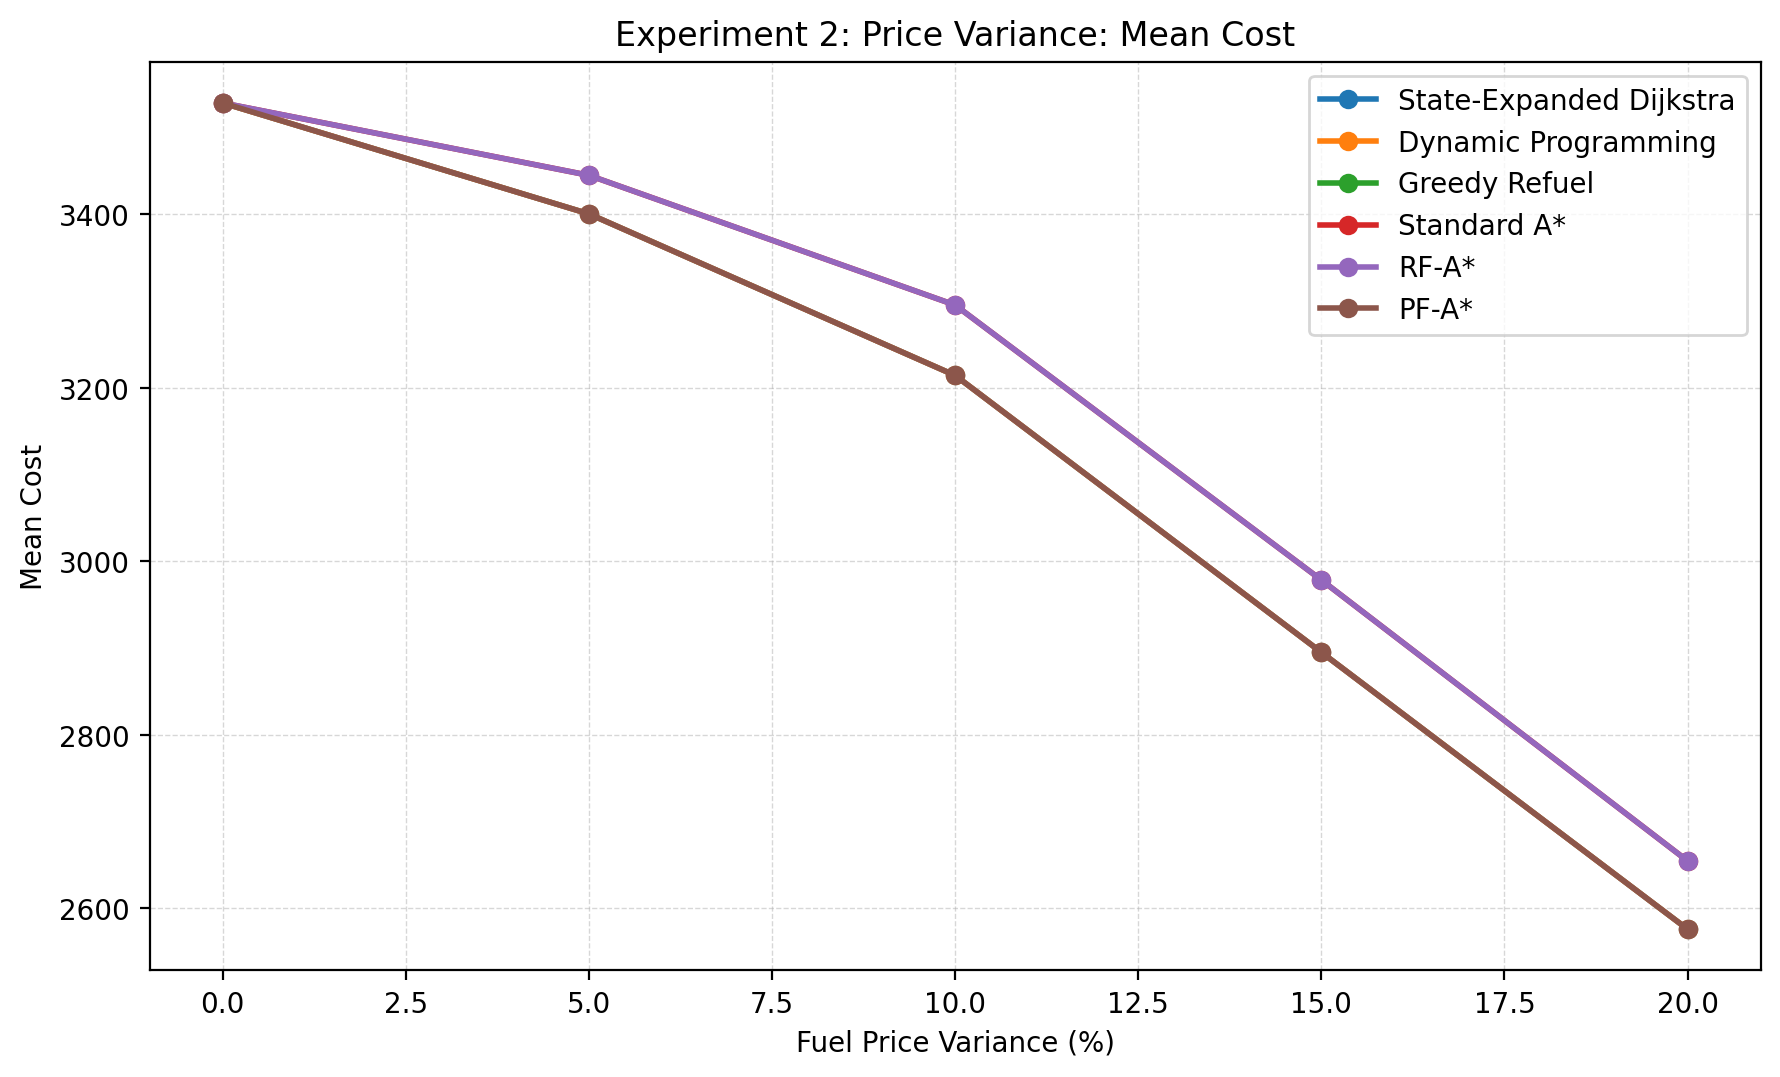
\includegraphics[width=0.90\textwidth]{../results/report_assets/exp2_price_variance/exp2_price_variance_cost.png}
      \caption{Experiment~2 mean cost under increasing fuel-price variance. Larger variance strengthens the value of cost-aware purchase decisions; PF-A*, Dynamic Programming, and State-Expanded Dijkstra coincide on the best cost curve.}
      \label{fig:curr_exp2_cost}
\end{figure}

\subsection*{Experiment 3: Tank Capacity}

Experiment~3 shows a clear cost--computation trade-off.
As tank capacity increased from 20\,L to 80\,L, the optimal mean cost fell from 3922.82 to 2185.84 because the vehicle gained more flexibility to defer purchasing to cheaper stations.
However, the larger tank also increased the effective state space for the exact methods: Dijkstra grew from 27.69\,ms at 20\,L to 567.22\,ms at 80\,L, while Dynamic Programming showed a similar increase.
PF-A* again preserved the optimal cost at every tested tank size, but with far lower runtime, rising only from 18.94\,ms to 120.80\,ms across the same range.

\begin{figure}[H]
      \centering
      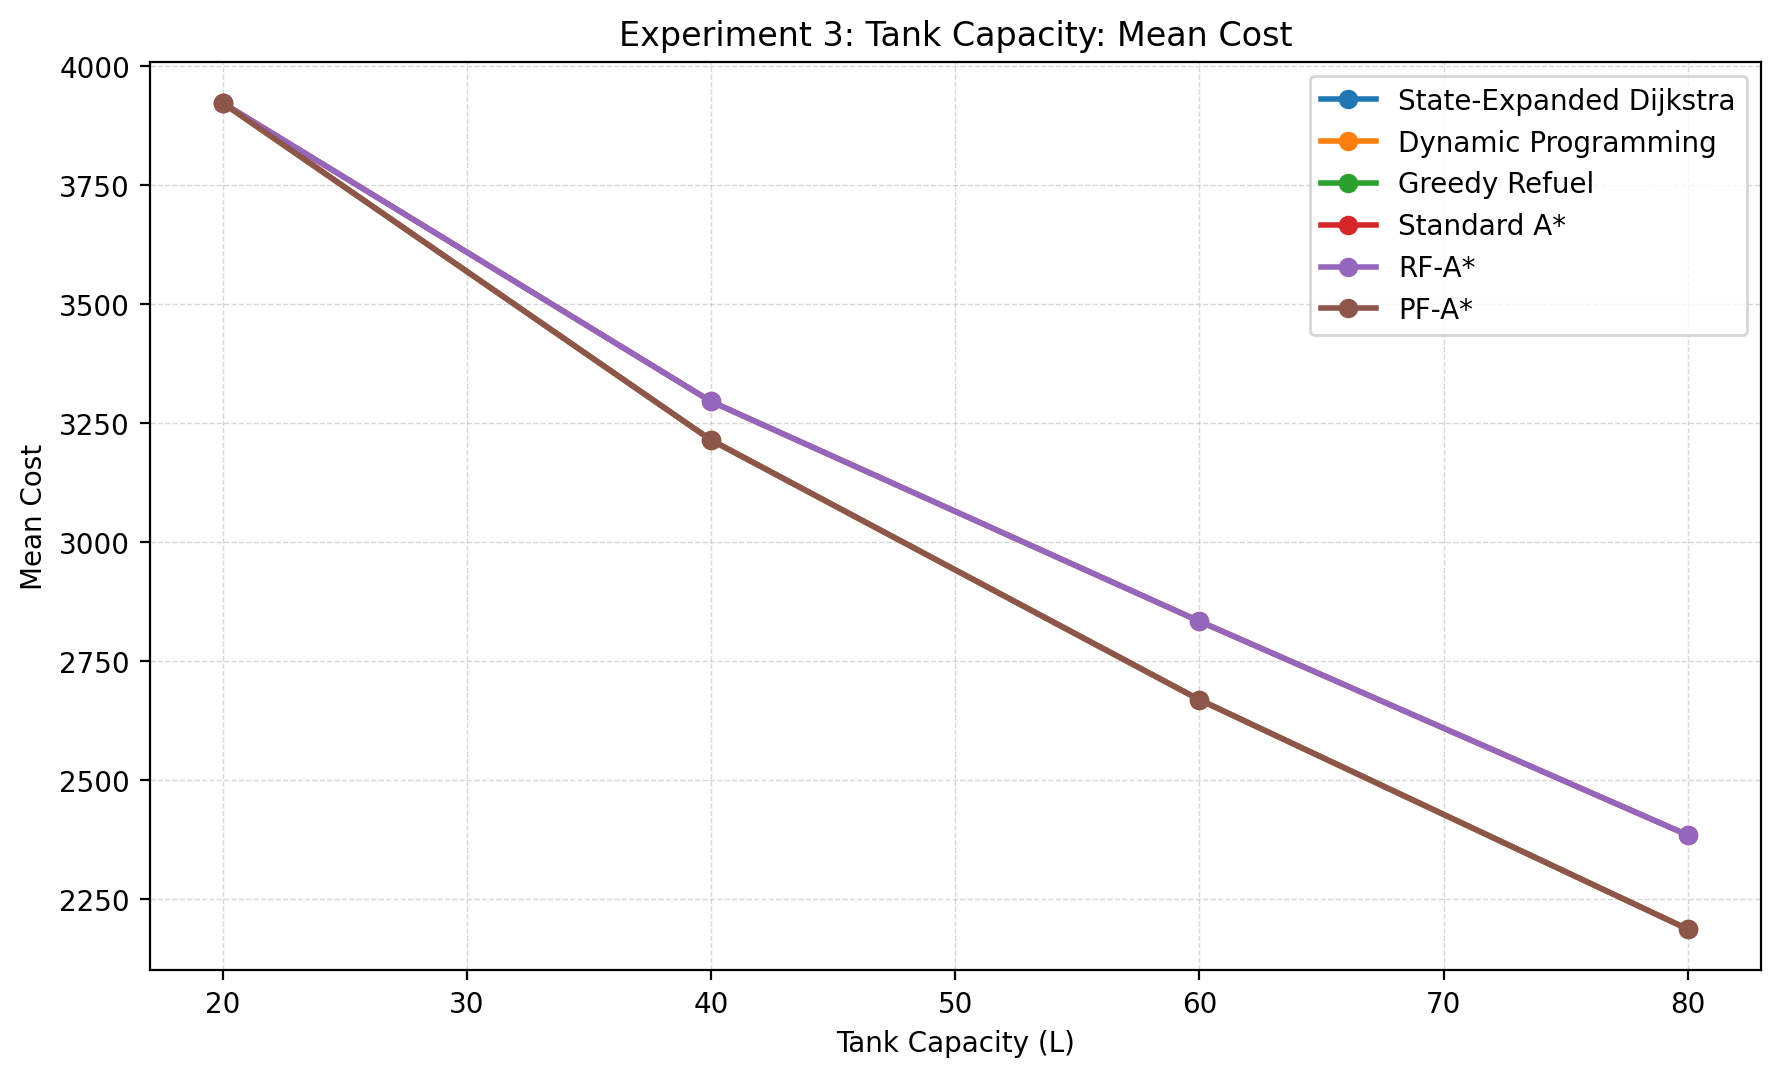
\includegraphics[width=0.90\textwidth]{../results/report_assets/exp3_tank_capacity/exp3_tank_capacity_cost.png}
      \caption{Experiment~3 mean cost as tank capacity varies. Larger tanks reduce the optimal fuel cost, but they also expand the search space for the exact state-expanded methods.}
      \label{fig:curr_exp3_cost}
\end{figure}

\subsection*{Experiment 4: Initial Fuel Level}

The initial-fuel experiment confirms that starting with more fuel reduces both cost and search effort.
For the optimal methods, mean cost decreased from 3848.58 at 10\,L initial fuel to 2831.54 at 40\,L.
PF-A* also became faster as the initial fuel level increased, improving from 71.60\,ms at 10\,L to 46.98\,ms at 40\,L.
This is consistent with the fact that higher initial fuel weakens the immediate need for costly early refuelling decisions and shrinks the number of states that need to be explored near the origin.

\begin{figure}[H]
      \centering
      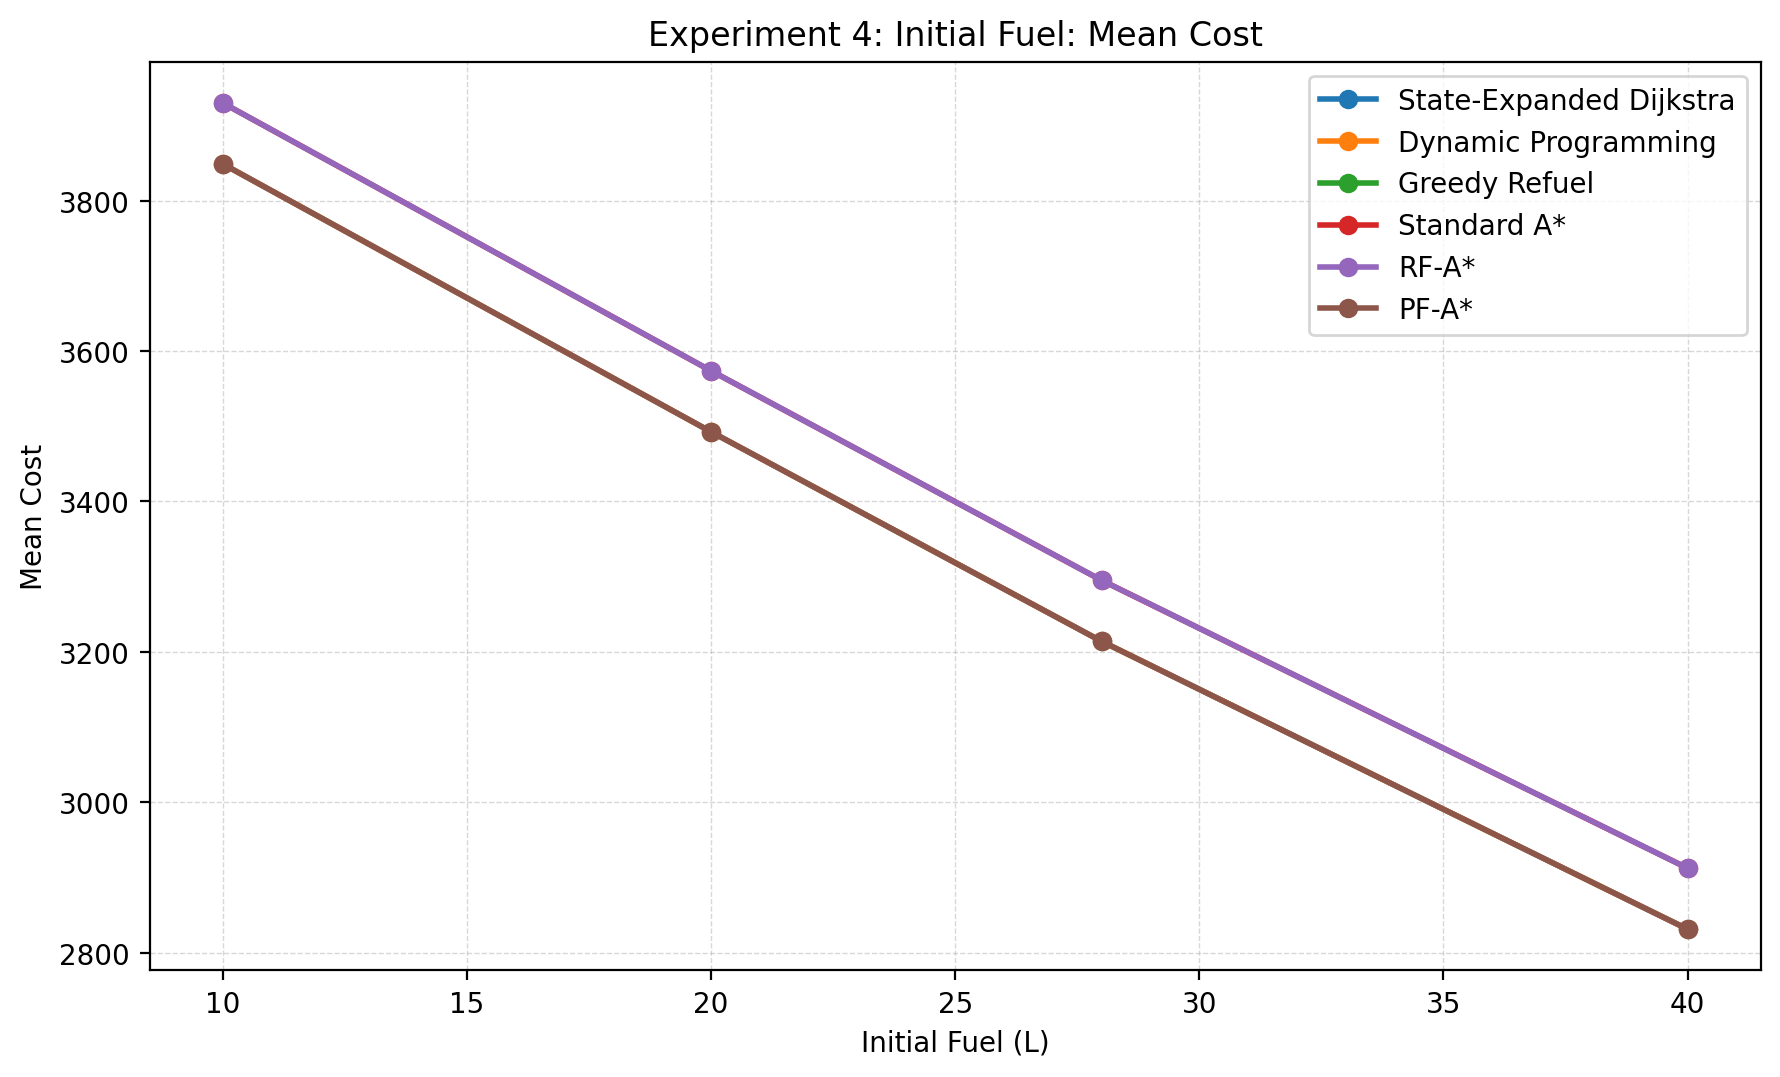
\includegraphics[width=0.90\textwidth]{../results/report_assets/exp4_initial_fuel/exp4_initial_fuel_cost.png}
      \caption{Experiment~4 mean cost as the initial fuel level varies. Higher initial fuel reduces the amount of expensive en-route purchasing and lowers the optimal total fuel expenditure.}
      \label{fig:curr_exp4_cost}
\end{figure}

\subsection*{Experiment 5: PF-A* versus RF-A*}

Experiment~5 is the central novelty experiment because it directly compares the proposed PF-A* heuristic against RF-A*.
Across all feasible configurations, PF-A* was markedly faster than RF-A*.
The average runtime over feasible configurations was 81.85\,ms for PF-A* compared with 394.83\,ms for RF-A*, a speedup of approximately 4.8$\times$.
At degree 5 and $\sigma=10\%$, PF-A* required only 2115 expanded states on average and completed in 59.92\,ms, while RF-A* expanded 18,507 states and required 475.48\,ms.
At degree 3, both algorithms were infeasible across all tested price-variance settings, indicating that the current sparse synthetic construction can disconnect or over-constrain the route.

An important observation from the current dataset is that PF-A* not only ran faster than RF-A* but also returned lower mean costs in every feasible configuration.
This differs from the theoretical expectation stated in Chapter~\ref{ch:experiments}, where both were expected to agree on the optimal cost.
Consequently, the RF-A* and Standard A* implementations now require targeted auditing before the final dissertation submission and before Experiment~6 is executed at full scale.

\begin{table}[H]
    \centering
    \caption{Representative Experiment~5 comparison at $\sigma=10\%$.}
    \label{tab:exp5_sigma10}
    \begin{tabular}{lcccc}
        \toprule
        Algorithm & Degree & Feasible (\%) & Mean Cost & Mean Runtime (ms) \\
        \midrule
        RF-A* & 5  & 100 & 3295.18 & 475.48 \\
        PF-A* & 5  & 100 & 3214.11 & 59.92 \\
        RF-A* & 10 & 100 & 2944.98 & 518.06 \\
        PF-A* & 10 & 100 & 2794.91 & 80.49 \\
        RF-A* & 20 & 100 & 2752.33 & 422.48 \\
        PF-A* & 20 & 100 & 2554.99 & 82.57 \\
        \bottomrule
    \end{tabular}
\end{table}

\begin{figure}[H]
      \centering
      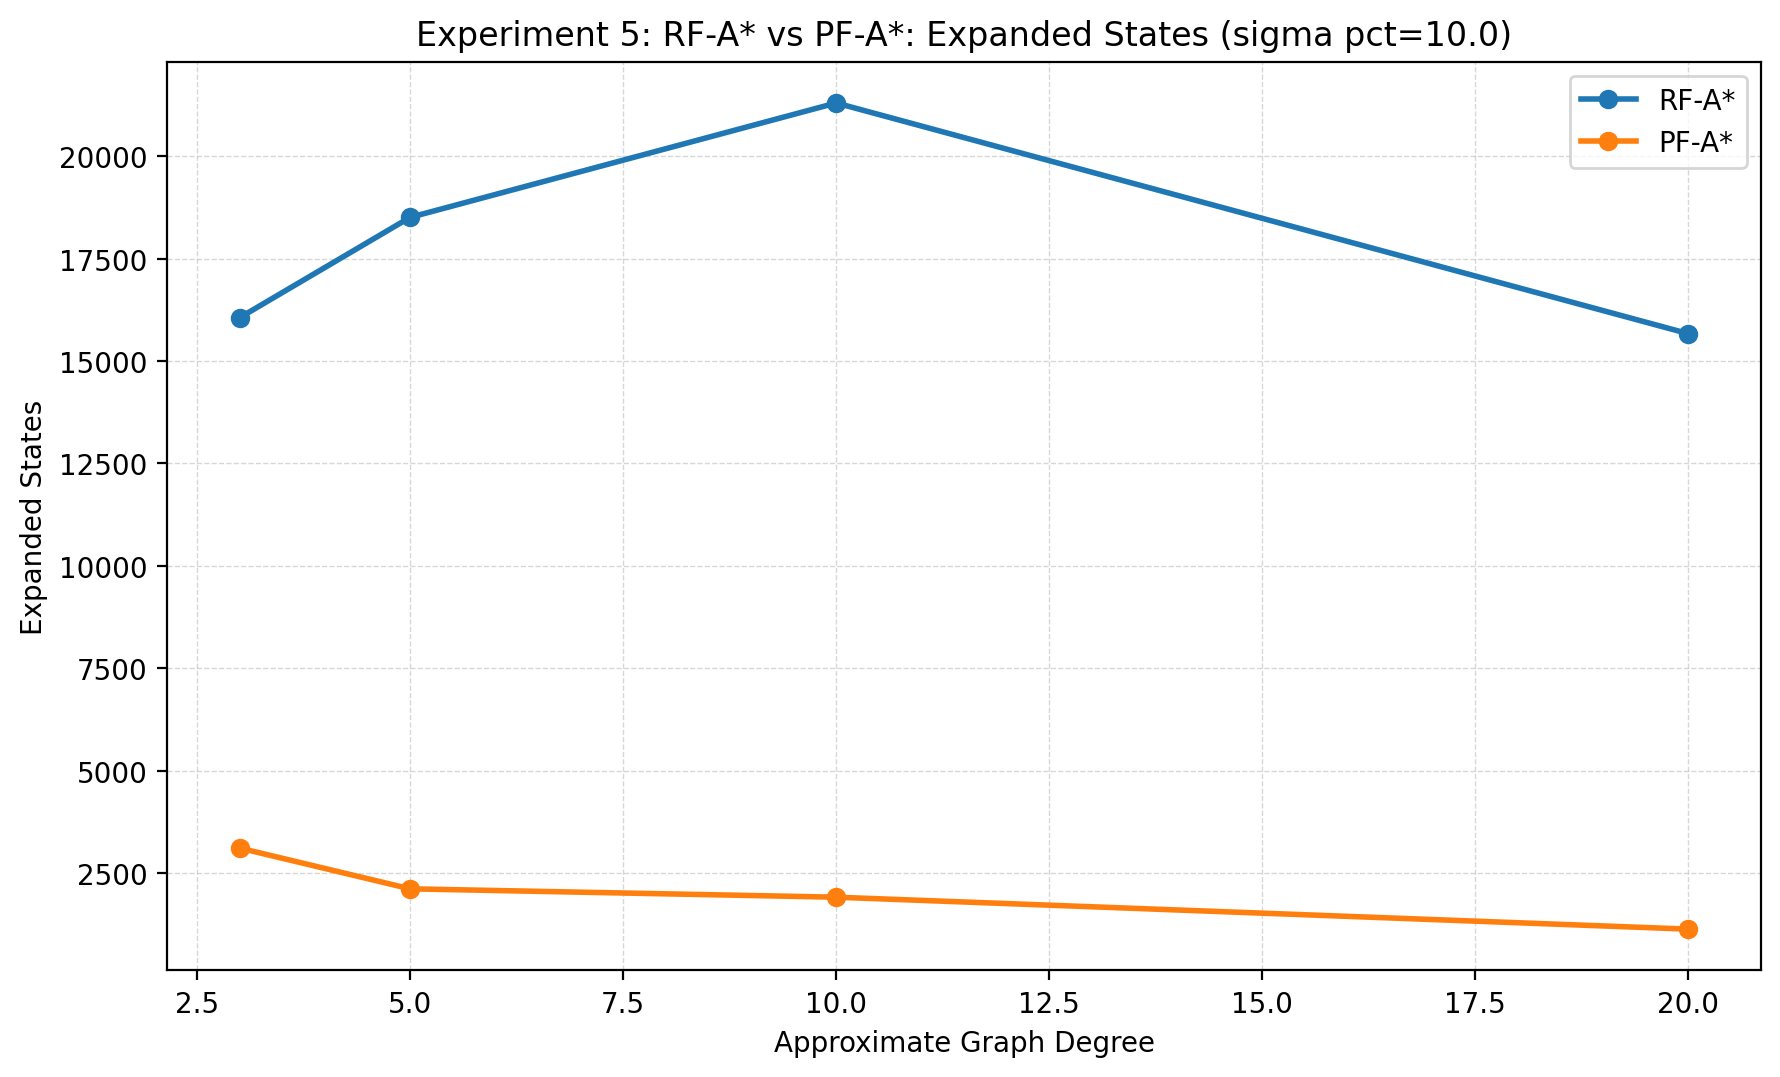
\includegraphics[width=0.90\textwidth]{../results/report_assets/exp5_rf_vs_pf/exp5_rf_vs_pf_expanded_states_sigma_pct_10_0.png}
      \caption{Experiment~5 node expansions for RF-A* and PF-A* at $\sigma=10\%$. PF-A* explores far fewer states in every feasible tested density regime.}
      \label{fig:curr_exp5_expanded}
\end{figure}

\subsection*{Experiment 7: Variable Purchase versus Full-Tank-Only}

Experiment~7 confirms the practical value of the variable-purchase model.
The variable-purchase State-Expanded Dijkstra solution was cheaper in every tested configuration, while the full-tank-only baseline was consistently faster.
Across the 16 tested $(\sigma, C)$ combinations, the full-tank-only model incurred an average cost penalty of 10.86\%, with observed penalties ranging from 1.19\% to 24.81\%.
At $\sigma=10\%$ and $C=80$\,L, for example, the full-tank-only strategy cost 2728.20 compared with 2185.84 for the variable-purchase optimum, a 24.81\% increase.
This experiment therefore provides strong synthetic evidence that modelling partial refuelling decisions yields meaningful monetary savings, even though it introduces additional computational overhead.

\begin{table}[H]
    \centering
    \caption{Representative Experiment~7 comparison at $\sigma=10\%$.}
    \label{tab:exp7_sigma10}
    \begin{tabular}{lccc}
        \toprule
        Tank capacity (L) & Variable-purchase cost & Full-tank-only cost & Cost gap (\%) \\
        \midrule
        20 & 3922.82 & 4137.17 & 5.46 \\
        40 & 3214.11 & 3611.20 & 12.35 \\
        60 & 2668.14 & 2799.09 & 4.91 \\
        80 & 2185.84 & 2728.20 & 24.81 \\
        \bottomrule
    \end{tabular}
\end{table}

\begin{figure}[H]
      \centering
      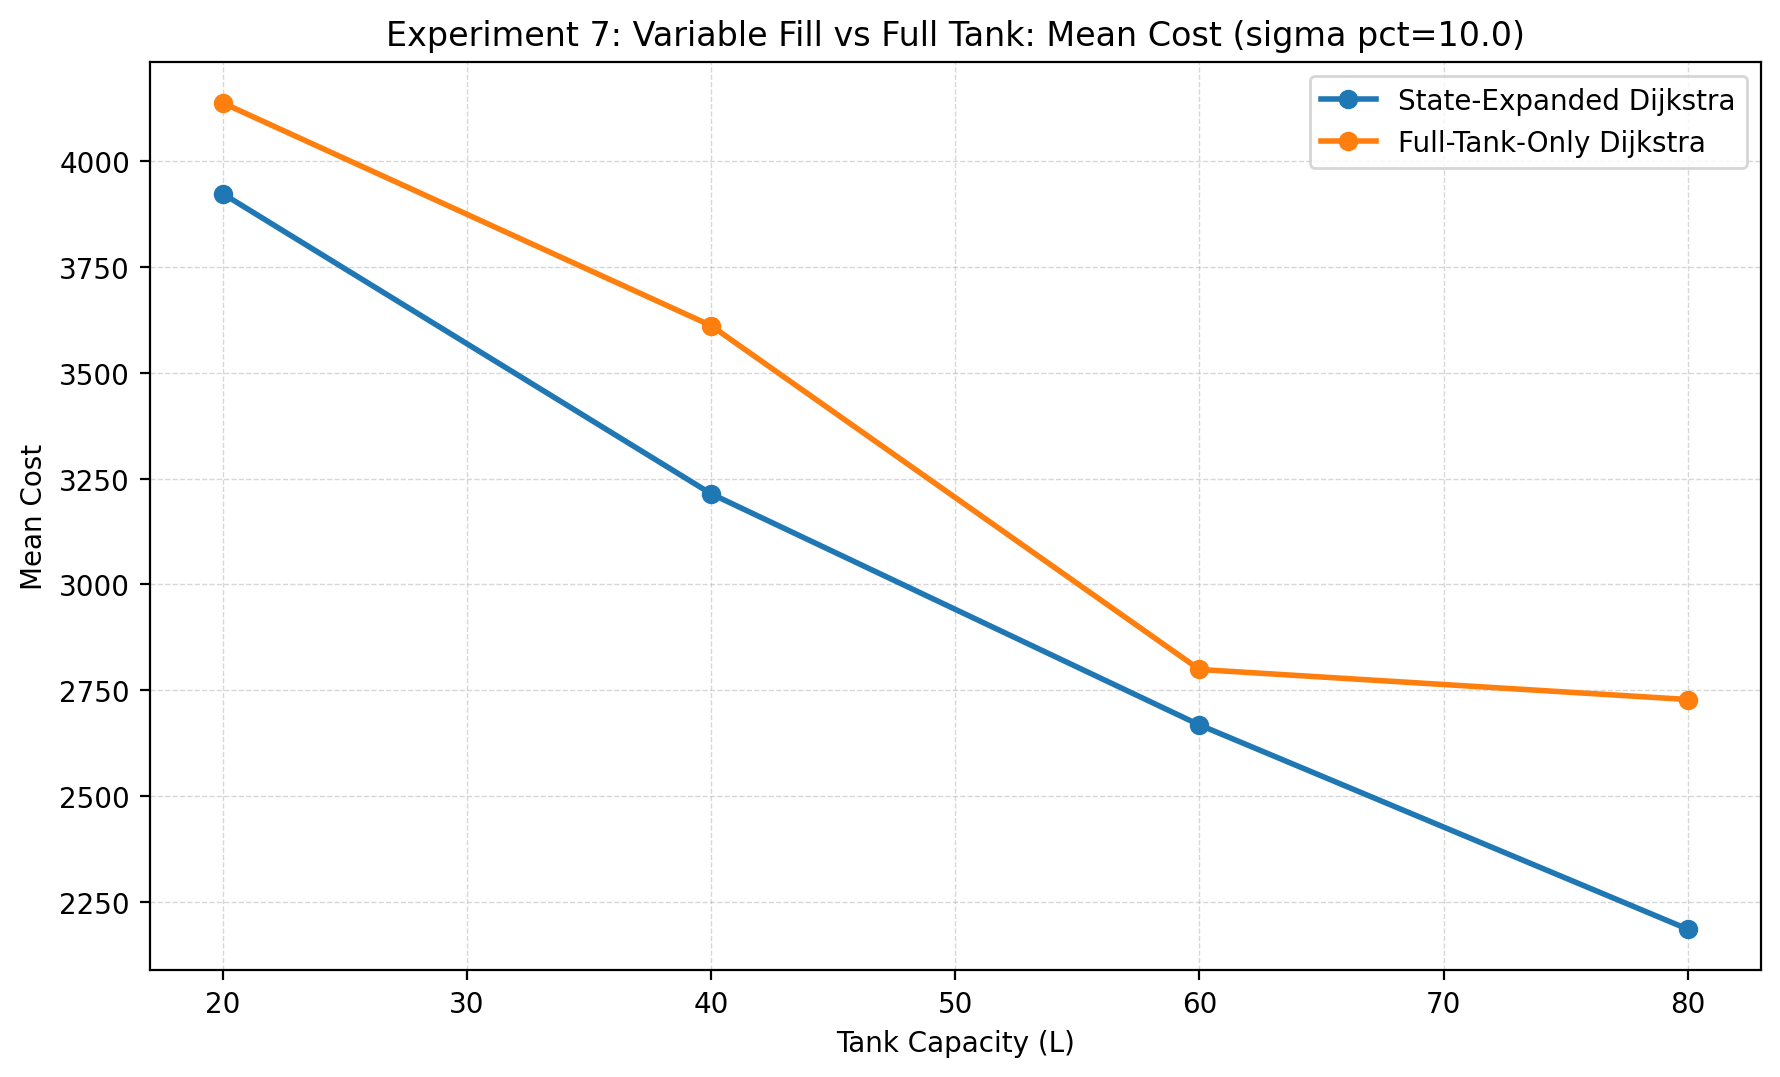
\includegraphics[width=0.90\textwidth]{../results/report_assets/exp7_variable_vs_full_tank/exp7_variable_vs_full_tank_cost_sigma_pct_10_0.png}
      \caption{Experiment~7 mean cost at $\sigma=10\%$ under the variable-purchase and full-tank-only models. The cost advantage of variable purchase remains visible across all tested tank capacities.}
      \label{fig:curr_exp7_cost}
\end{figure}

\subsection*{Summary of Current Findings}

The present synthetic results support three main conclusions.
First, PF-A* is already the strongest all-round algorithm in the current implementation: it matches the best observed costs in Experiments~1--4 while substantially reducing runtime relative to Dijkstra and Dynamic Programming.
Second, the value of the fuel-aware purchase model is now empirically clear, with Experiment~7 showing consistent and sometimes large penalties for the full-tank-only baseline.
Third, the current experiments also exposed an implementation-level issue: Standard A* and RF-A* do not currently match the best observed costs, even though they were expected to do so in the experimental design.
That discrepancy is not hidden by the present report; rather, it now forms an explicit part of the remaining work before the final dissertation.

\section{Work Remaining}

The remaining work of the project is summarised as follows:

\begin{enumerate}
    \item Audit the Standard A* and RF-A* implementations against the exact Dijkstra and Dynamic Programming baselines, since the current synthetic results show persistent cost gaps where equality had been expected.
    \item Execute the full strict-profile synthetic experiment suite, comprising 10,000 timed runs and 200 warm-up iterations for each configuration, and collect the final dataset of results.
    \item Perform the planned statistical analysis using Wilcoxon signed-rank tests with Bonferroni correction.
    \item Finalise the dissertation-quality visualisations and tables for the strict-profile synthetic results.
    \item Conduct the final real-world evaluation on Thai routes in Experiment~6.
\end{enumerate}

\section{Plan for Experiment~6 (Real Thai Routes)}

Experiment~6 is now the main remaining empirical milestone.
Based on the current synthetic findings, the real-route evaluation should be executed in a staged and auditable manner rather than as a single end-stage run.

\begin{enumerate}
    \item \textbf{Validate the real-route data pipeline.}
          Re-check the OSM-derived road graph, station extraction, and corridor definitions for Bangkok--Chiang Mai, Bangkok--Phuket, and Bangkok--Khon Kaen.
          Confirm that every station used in the experiment is reachable in the drivable network and that the source and destination nodes are correctly anchored.

    \item \textbf{Freeze the price-assignment procedure.}
          Finalise how provincial or regional fuel prices are attached to stations, document fallback rules for missing price records, and record the exact snapshot used in the experiment for reproducibility.

    \item \textbf{Construct per-corridor benchmark instances.}
          For each corridor, export a cleaned route graph containing station prices, road-segment distances, source and destination identifiers, and the fixed vehicle parameters ($C=40$\,L, $f_0=28$\,L, $\eta=10$\,km/L).
          Run feasibility checks to ensure that each corridor admits at least one valid route.

    \item \textbf{Run a correctness pass before the full benchmark.}
          Execute State-Expanded Dijkstra, Dynamic Programming, PF-A*, RF-A*, and the full-tank-only baseline on each corridor once and compare returned paths, costs, and feasibility.
          This step is especially important in light of the current synthetic discrepancy for RF-A* and Standard A*.

    \item \textbf{Execute the real-route benchmark sweep.}
          After correctness validation, run the selected real-route algorithms repeatedly under the final evaluation profile and store per-run results in the same tabular format already used for the synthetic pipeline.

    \item \textbf{Analyse cost savings and route structure.}
          Report total fuel cost, runtime, and state expansions for each corridor, and compare variable-purchase routing against the full-tank-only baseline.
          In addition, inspect where partial refuelling decisions occur geographically, since these qualitative route differences are likely to be important in the final dissertation discussion.
 \end{enumerate}

\section{Expected Contributions}

This project is expected to make four principal contributions.

\begin{enumerate}
    \item \textbf{Algorithmic contribution: Partial-Fill A* (PF-A*).}
          PF-A* introduces a fuel-level-aware heuristic extension of RF-A* by replacing the global-$p_{\min}$ heuristic with the state-dependent heuristic $h_{\mathrm{PF}}(v,f)$.
          To the best of the author's knowledge, this is the first heuristic for the Gas Station Problem that jointly incorporates the current fuel level of the vehicle and the cheapest reachable station from the current state.
          Its admissibility and consistency have been formally proved, and its principal contribution lies in its expected practical reduction of node expansions on large road networks with realistic price variation.

    \item \textbf{Empirical evaluation on real Thai road data.}
          The project will provide an empirical comparison of State-Expanded Dijkstra, Greedy, DP, RF-A*, and PF-A* on Thailand's real fuel station network using actual road topology and provincial fuel price data.
          This evaluation will also examine the theoretical claim of Khuller et al.\ that partial-refuelling strategies can yield savings of 5--15\% relative to full-tank-only approaches.

    \item \textbf{Dataset and reproducibility contribution.}
          The project will produce a curated Thailand fuel-station graph that integrates road topology with fuel price information, together with a configurable synthetic benchmark generator supporting controlled variation in station density, price variance, tank capacity, and origin-destination distance.
          In addition, a reproducible benchmarking environment will be provided to support repeatable evaluation.

    \item \textbf{Prototype system contribution.}
          As a longer-term extension, the project aims to develop a web-based route-planning demonstration capable of visualising optimal fuel-aware routes on interactive Thai map data.
          This prototype is intended to illustrate the practical applicability of the proposed methods in a real deployment context.
\end{enumerate}
